\chapter{Motivación teórica}
\label{ch:theory}
% \epigraph{\emph{\enquote{Nothing in life is to be feared. It is only to be understood. Now is the time to understand more, so that we may fear less}}}{Marie Curie}


Esta tesis se centra en la búsqueda de nuevas partículas predichas por diferentes escenarios más allá del \ac{SM}. En este capítulo se presenta un resumen de los principales conceptos del \ac{SM} utilizados a lo largo de esta tesis. Además, se describen las interacciones hadrónicas en una colisión \pp y en el proceso de producción de fotones \textit{prompt}.
A continuación, en \Sect{\ref{sec:theory:bsm}} se ofrece una vista general de las limitaciones actuales del \ac{SM} y cómo, con modelos de física \ac{BSM}, se pretenden resolver estos problemas.
Por último, en la \Sect{\ref{sec:theory:mc_simulation}}, el capítulo termina con cómo se simulan estos procesos del \ac{SM} utilizando \ac{MC}, mostrando los diferentes pasos y herramientas para hacerlo.




\section{El Modelo Estándar}
\label{sec:theory:sm}

El \acf{SM} de física de partículas es la teoría matemática que describe todas las partículas elementales conocidas y sus interacciones.
La teoría se ha ido desarrollando a lo largo de varias decadas y tras numerosos experimentos que respaldaron sus predicciones, se ha convertido en la teoría más completa de la física de partículas.

El \ac{SM} logra describir tres de las cuatro fuerzas fundamentales de la naturaleza: las interacciones \ac{EM}, débil y fuerte, las cuales actúan en distintos rangos.
La gravedad, la cuarta fuerza de la naturaleza, aunque no está incluida en el \ac{SM}, es la más débil de las interacciones y tiene un alcance infinito.
Las tres fuerzas fundamentales del \ac{SM} resultan del intercambio de partículas que pertenecer al grupo de \textit{bosones}. Las partículas de materia, los \textit{fermiones}, interactúan entre ellas transfiriendo cantidades discretas de energía a través del intercambio de estos bosones.



\subsection{Partículas elementales y sus interacciones}
\label{subsec:theory:sm:particles_interaction}

Según el \ac{SM}, toda la materia está formada por fermiones, que son partículas que siguen la estadística de Fermi-Dirac y tienen spin semi-entero. Estos fermiones interactúan entre sí mediante el intercambio de bosones, que son partículas de spin entero, siguiendo la estadística de Bose-Einstein. Hasta la fecha no ha habido ningún experimento capaz de encontrar pruebas de que estas partículas tengan estructura interna.

\begin{figure}[ht!]
    \centering
    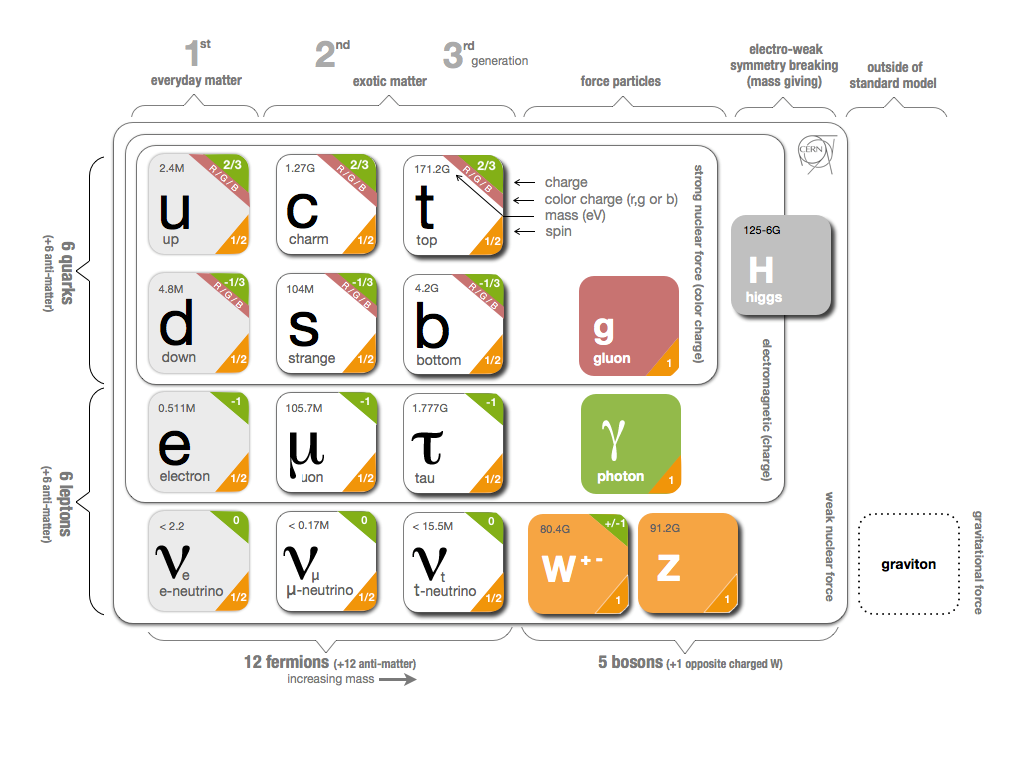
\includegraphics[width=\linewidth]{2_theory/sm}
    \caption{Partículas del \ac{SM} y sus propiedades. Todos los fermiones participan en la interacción débil, pero sólo los quarks interaccionan con los gluones, mientras que tanto los quarks como los leptones cargados interaccionan mediante la fuerza \ac{EM}. Los neutrinos, al ser neutros e incoloros, sólo interaccionan con los bosones \Wboson y \Zboson a través de la fuerza débil. Por último, el gravitón, aunque aún no se ha descubierto, debería ser el correspondiente portador de la fuerza gravitatoria. Extraído de la \Refn{\cite{SM_diagram}}.}
    \label{fig:theory:sm:particles_interaction:particles}
\end{figure}

Los fermiones se dividen en dos tipos de partículas elementales: los leptones y los quarks. Existen seis leptones clasificados según su carga que se dividen en tres familias o generaciones, ordenadas en función de su masa. Las partículas de las generaciones superiores tienen mayor masa y son muy inestables, decayendo en leptones de generaciones inferiores. Por esta razón, la materia se construye a partir de leptones de primera generación. Los leptones son: electrón (\(e\)), muón (\(\mu\)) y tau (\(\tau\)), con sus respectivos neutrinos: neutrino electrón (\(\nu_{e}\)), neutrino muón (\(\nu_{\mu}\)) y neutrino tau (\(\nu_{\tau}\)).
También hay seis antileptones que tienen carga eléctrica opuesta a la de los leptones. El electrón, el muón y el tau tienen carga eléctrica y una masa considerable, mientras que los neutrinos son eléctricamente neutros y tienen una masa muy pequeña (aunque en el \ac{SM} es estrictamente cero).

Del mismo modo, hay seis sabores (flavours) de quarks, también con sus respectivas antipartículas: up (\(u\)), down (\(d\)), charm (\(c\)), strange (\(s\)), top (\(t\)) y bottom (\(b\)). Los quarks también presentan otra propiedad que es el número cuántico de color y sólo se mezclan de tal manera que forman objetos sin color. En la \Fig{\ref{fig:theory:sm:particles_interaction:particles}} se muestra un resumen de los quarks y sus propiedades.


Cada una de las tres fuerzas en el \ac{SM} se describe mediante una \ac{QFT}.
La fuerza fuerte, mediada por gluones sin masa, es responsable de la interacción entre los quarks que aunque no tienen carga eléctrica poseen carga de color. A pesar de que estos no tienen masa, la interacción fuerte se hace más fuerte a bajas energías, confinando quarks y gluones dentro de hadrones debido a la propiedad de libertad asintótica y a la propiedad de \textit{confinamiento}, las cuales serán discutidas más adelante.
La fuerza \ac{EM} entre partículas cargadas está mediada por fotones. Los fotones no tienen masa y, en consecuencia, la interacción tiene un alcance infinito.
Por último, la interacción débil está mediada por los bosones masivos \Wboson y \Zboson, que dan lugar a interacciones de corto alcance. Las propiedades fundamentales de estos bosones también se muestran en la \Fig{\ref{fig:theory:sm:particles_interaction:particles}}.









\subsection{Breve descripción matemática del Modelo Estándar}
\label{subsec:theory:sm:mathematical}

El \ac{SM} es una teoría de campos renormalizable basada en simetrías locales que proporciona una descripción de las partículas fundamentales y sus interacciones: la fuerte, la débil y la \ac{EM}. Estas interacciones aparecen por el requisito de que la teoría es invariante bajo transformaciones gauge locales del grupo de simetría:
\begin{equation*}
    SU(3)_{C} \times SU(2)_{L} \times U(1)_{Y},
\end{equation*}
donde \(Y\) es la hipercarga, \(L\) la helicidad izquierda y \(C\) la carga de color, y representan las cantidades conservadas del grupo de simetría. Cada transformación gauge local puede ser absorbida dentro de un campo de gauge, con las excitaciones de los campos gauge llamadas bosones gauge. El sector \ac{EW} del \ac{SM} \(SU(2)_{L} \times U(1)_{Y} \to U(1)_{\text{EM}}\) describe las interacciones débil y \ac{EM}, tras el mecanismo de ruptura espontánea de simetría en virtud del potencial de Higgs. El grupo no abeliano \(SU(3)_C\), con carga de color, describe las interacciones fuertes entre quarks y gluones y la teoría se conoce como \ac{QCD}~\cite{Ellis-1996-book}.

En principio, las partículas incluidas en el \ac{SM} carecen de masa a diferencia de las partículas observadas en la naturaleza. Aunque las ecuaciones de la interacción \ac{EW} describen correctamente partículas como el fotón, no dan cuenta de las masas de los bosones \Wboson y \Zboson. Para solucionar este problema se introdujo el concepto de \ac{EWSB}, conocido como mecanismo de Brout-Englert-Higgs~\cite{Higgs-1964_1,Higgs-1964_2,Higgs-1966,Englert_Brout-1964}. Este mecanismo explica cómo los bosones \Wboson y \Zboson adquieren masa a través de la ruptura espontánea de la simetría \ac{EW}, causada porque el campo escalar de Higgs adquiere un \ac{VEV} distinto de cero. Además, predice la existencia de una nueva partícula escalar, dando lugar a un nuevo bosón masivo de spin 0, denominado bosón de Higgs. Esta partícula fue confirmada experimentalmente en 2012 por las colaboraciones \ac{ATLAS}\acused{ATLAS} y \ac{CMS}\acused{CMS} en el \ac{LHC}\acused{LHC}, con una masa medida de \(125.11 \pm 0.11~\gev\)~\cite{ATLAS-HiggsObservation,CMS-HiggsObservation,ATLAS-Higgs-2024}.








\subsubsection{The interaccón \acl{EW}}

Las interacciones \ac{EW} satisfacen la simetría de gauge del grupo \(SU(2)_L \times U(1)_Y\). El grupo \(SU(2)_L\), llamado isospín débil actúa sólo sobre los fermiones de quiralidad izquierda y \(U(1)_Y\) es el grupo de hipercarga que actúa sobre ambas quiralidades de forma vectorial.
El grupo \(SU(2)_L \times U(1)_Y\) tiene cuatro generadores, de los cuales tres pertenecen al isospín débil: \(T_i = \frac{\sigma_i}{2}\), siendo \(i = 1,\, 2,\, 3\) y \(\sigma_i\) las matrices de Pauli y uno al grupo de hipercarga: \(\frac{Y}{2}\). Los fermiones izquierdos se transforman como dobletes bajo \(SU(2)_L\), \(f_L \ra e^{i T_i \theta_i} f_L\) con
\begin{equation}
    f_L = \mqty( \nu_L\\ e_L ), \mqty( u_L\\ d_L ), \dots,
\end{equation}
mientras que los fermiones derechos se transforman como singletes \(f_R \ra f_R\) con
\begin{equation}
    f_R = e_R, \, u_R,\, d_R, \dots.
\end{equation}
Esta distinción entre izquierdos y derechos implica que la teoría \(SU(2)_L \times U(1)_Y\) es una teoría quiral.
Por otro lado, la carga eléctrica está relacionada con la tercera componente del isospín débil \(T_3\) y la hipercarga \(Y\), según la fórmula de Gell-Mann Nishijima:
\begin{equation}
    Q = T_3 + \frac{Y}{2}
\end{equation}

El número de bosones de gauge asociados coincide con el número de generadores del grupo de simetría. Para el isospín débil hay 3 bosones \(SU(2)_L\): \(W_{\mu}^1,\, W_{\mu}^2,\, W_{\mu}^3\), y para \(U(1)\) se tiene un bosón de hipercarga: \(B_{\mu}\).
La simetría global \(SU(2)_L \times U(1)_Y\) se convierte en local, sustituyendo en la lagrangiana la derivada de los campos por la derivada covariante:
\begin{equation}
    \label{eq:theory:sm:mathematical:ew:covariant_derivative}
    D_{\mu} = \partial_{\mu} - ig \frac{\tau^i}{2} W_{\mu}^i - i g' \frac{Y}{2} B_{\mu},
\end{equation}
donde \(g\) es la constante de acoplamiento de \(SU(2)_L\) y \(g'\) de \(U(1)_Y\).

La densidad lagrangiana \ac{EW} puede escribirse entonces como la suma del lagrangiano fermiónico con las interacciones de gauge y los términos cinéticos para los campos de gauge introducidos:
\begin{equation}
    \mathcal{L}_{\text{EW}} = 
    - \frac{1}{4} F_{\mu\nu}^i F^{\mu\nu}_i
    - \frac{1}{4} B_{\mu\nu} B^{\mu\nu}
    + \sum_{f = \ell, q} \bar{f} i \gamma^{\mu} D_{\mu} f,
\end{equation}
donde los tensores de campo de Yang-Mills \(F_{\mu\nu}^i\) para \(SU(2)_L\) y \(B_{\mu\nu}^i\) para \(U(1)_Y\) se definen como:
\begin{gather}
    F_{\mu\nu}^i = \partial_{\mu} W_{\nu}^i  -  \partial_{\nu} W_{\mu}^i + g \epsilon_{ijk} W_{\mu}^jW_{\nu}^k \\
    B_{\mu\nu} = \partial_{\mu} W_{\nu}  -  \partial_{\nu} W_{\mu}.
\end{gather}




\subsubsection{El mecanismo de Higgs}

La formulación hasta ahora descripta no incluye en las masas de ninguna de las partículas. Esto se debe a que al agregar términos de masa explícitos al lagrangiano (como por ejemplo \(m \psi \hat{\psi}\) o \(m_B^2 B^{\mu}B_{\mu}\)), el mismo pierde la invarianza \ac{EW}. La forma de incluir masas a la teoría es mediante el mecanismo de Higgs. Para ello se asume la existencia de un campo de spin 0, denominado campo de Higgs. El mismo es un doblete en el espacio \(SU(2)\) y tiene hipercarga no nula en \(U(1)\), pero es un singlete en el espacio de color. Los bosones de gauge y los fermiones pueden interactuar con este campo, y en su presencia dejan de tener masa nula. Si bien el Lagrangiano conserva la simetría \(SU(2)\) y \(U(1)\), el estado fundamental no, en lo que se denomina un rompimiento espontáneo de simetría.

El sector de Higgs del Lagrangiano viene dado por:
\begin{equation}
    \mathcal{L}_{\text{Higgs}} = \left(D^{\mu} \phi\right)^{\dagger} \left(D_{\mu} \phi\right) - V(\phi)
\end{equation}
donde \(\phi\) es un campo escalar complejo en la representación \(SU(2)\):
\begin{equation}
    \Phi = \mqty( \phi_{+} \\ \phi_0 ) = \frac{1}{\sqrt{2}} \mqty(\phi_1 + i \phi_2 \\ \phi_3 + i \phi_4),
\end{equation}
con hipercarga \(U(1)\) \(Y=+1\), donde \(\phi_{+}\) y \(\phi_{0}\) son complejos con carga eléctrica \(+1\) y \(0\), respectivamente y la derivada covariante viene dada por la \Eqn{\ref{eq:theory:sm:mathematical:ew:covariant_derivative}}. La razón de tener la simetría adicional \(U(1)_Y\) es para que la teoría produzca un bosón de gauge sin masa asociado al fotón. Se requiere que el potencial de Higgs \(V(\phi)\) tenga la forma
\begin{equation}
    V(\phi) = -\mu^2 \phi^{\dagger} \phi + \lambda \left(\phi^{\dagger} \phi\right)^2
\end{equation}
para garantizar la renormalizabilidad de la teoría y la invariancia de \(SU(2)\) y \(U(1)\). El parámetro \(\lambda\) tiene que ser positivo para que el potencial tenga un mínimo, de forma que el comportamiento del campo venga determinado entonces por \(\mu\). Para \(\mu^2 > 0\), el campo genera un \ac{VEV} distinto de cero (\(v := \phi^{\dagger} \phi\)) que rompe espontáneamente la simetría. El potencial \(V(\phi)\) tiene la forma conocida de un sombrero mexicano con infinitos estados degenerados con energía mínima que satisface \(v = \sqrt{-\mu^2/\lambda}\). De estos infinitos estados, es habitual utilizar:
\begin{equation}
    \expval{\Phi} = \frac{1}{\sqrt{2}} \mqty(0\\v)
\end{equation}
con \(\phi_1 = \phi_2 = \phi_4 = 0\), \(\phi_3 = v\).

Para estudiar el espectro de partículas, se estudia el campo alrededor del mínimo utilizando una expansión en la dirección radial:
\begin{equation}
    \phi = \frac{1}{\sqrt{2}} \mqty(0 \\ v + H(x)),
\end{equation}
donde \(H(x)\) son excitaciones del estado fundamental alrededor del mínimo pero en la dirección radial del potencial.
Debido a la invariancia de gauge del potencial para excitaciones alrededor de los mínimos de la circunferencia y de acuerdo con el teorema de Goldstone, uno debería en principio tener tres bosones escalares sin masa asociados a los grados de libertad no radiales del campo. La arbitrariedad de gauge permite que los bosones de Goldstone sean absorbidos por los bosones \Wboson y \Zboson (proporcionan las polarizaciones longitudinales adquiridas por los campos gauge). El desarrollo en la dirección radial da la masa de la excitación \(H\), \(\sqrt{2\lambda}\nu\) que es la masa del bosón de Higgs, y los acoplamientos cúbicos y cuárticos de este bosón. De esta manera, las masass de los bosones del \ac{SM} tienen la forma:
\begin{align}
    m_{g} &= 0\\
    m_{\gamma} &= 0\\
    m_{\Wboson} & = \frac{g v}{2}\\
    m_{\Zboson} & = \frac{g}{2} \sqrt{g^2 + g'^2}\\
    m_{H} & = \sqrt{2\lambda}\nu
\end{align}

Los términos de acoplamiento tipo Yukawa al campo de Higgs dan masas a los fermiones del \ac{SM}:
\begin{equation}
    \mathcal{L}_{\text{Yuk}} = g_f \left(\bar{\psi}_L \phi \psi_R + \phi^{\dagger} \bar{\psi}_R \psi_L\right),
\end{equation}
siendo este una invariante \(SU(2)\). La constante de acoplamiento \(g_f\) describe el acoplamiento entre el doblete de Higgs y los fermiones. Haciendo una expansión del campo similar a la realizada anteriormente y sustituyendo en el Lagrangiano de Yukawa, se obtienen términos que indican las masas de los fermiones como
\begin{equation}
    m_f = \frac{g_f v}{\sqrt{2}}.
\end{equation}


\subsubsection{La interacción fuerte}
\label{subsubsec:theory:sm:mathematical:qcd}

El enorme esfuerzo por describir el gran espectro de resonancias de mesones y bariones que se descubrieron durante la década de 1950, llevó a Gell-Mann y Zweig a proponer en 1964 el modelo de los quarks~\cite{Gellmann-1964,Zweig-1964_1,Zweig-1964_2}, que afirma que los hadrones son en realidad compuestos de constituyentes más pequeños. Zweig denominó a las partículas elementales \textit{aces} mientras que Gell-Mann las llamó \textit{quarks}, pero finalmente la teoría pasó a llamarse modelo de los quarks.

El modelo de los quarks se formalizó en la teoría de \ac{QCD} con quarks que llevan un número cuántico adicional llamado carga de color, \(C=R,G,B\). Sin carga de color, los quarks dentro de algunos hadrones existirían en estados cuánticos simétricos, en violación del principio de exclusión de Pauli.
La teoría satisface la simetría de gauge del grupo \(SU(3)_C\), que tiene ocho generadores \(T^a = \frac{\lambda_{\alpha\beta}^a}{2}\), siendo \(\alpha\) y \(\beta\) los índices de color y \(\lambda_{\alpha\beta}^a\) las ocho matrices de Gell-Man (\(a=1,2,\dots,8\)). Estos ocho generadores introducen ocho nuevos campos de gauge cuyos bosones asociados son los gluones.
Los mesones y bariones, hadrones compuestos por dos y tres quarks respectivamente, son singletes \textit{blancos} (carga de color neutro) de \(SU(3)_C\).

La simetría local \(SU(3)_C\) se obtiene sustituyendo en la lagrangiana las derivadas covariantes
\begin{equation*}
    D_{\mu} = \partial_{\mu} - i g_s \sum_{a=1}^{8} \frac{\lambda_{\alpha\beta}^a}{2} G_{\mu}^a,
\end{equation*}
donde \(g_s\) es la constante de acoplamiento \ac{QCD} desnuda y suele sustituirse por \(\alpha_s = g_s^2 / 4\pi\). El tensor de campo de Yang-Mills \(G_{\mu\nu}^a\) para el grupo \(SU(3)_C\) puede escribirse como
\begin{equation*}
    G_{\mu\nu}^a = \partial_{\mu} G_{\nu}^a - \partial_{\nu} G_{\mu}^a + g_s f_{abc} G_{\mu}^b G_{\nu}^c,
\end{equation*}
donde \(f_{abc}\) son las constantes de estructura de \(SU(3)\). Es importante observar que el último término de la ecuación anterior describe la autointeracción de los gluones, responsable de la naturaleza no abeliana de \ac{QCD}.
La densidad lagrangiana \ac{QCD} viene dada entonces por:
\begin{align*}
    \mathcal{L}_{\text{SM}} \supset \mathcal{L}_{\text{QCD}}
    &=
        -\frac{1}{2} \Tr\left\{G_{\mu\nu}G^{\mu\nu}\right\}
        + 
        \sum_{\text{flavours}} i \bar{q}_f \gamma^{\mu} D_{\mu} q_f\\
    &=
        -\frac{1}{4} \sum_{a=1}^{8} G_{\mu\nu}^a G^{\mu\nu}_a
        + 
        \sum_{\text{flavours}} i \bar{q}_f \gamma^{\mu} D_{\mu} q_f
\end{align*}

\paragraph{Renormalización}

Como se ha mencionado, el \ac{SM} es una \ac{QFT} renormalizable. A continuación se detalla brevemente a qué se refiere este término. Los efectos de orden superior introducen correcciones cuánticas, por ejemplo, en el cálculo de los acoplamientos en el \ac{SM}, que deben tenerse en cuenta. Al mismo tiempo, las partículas en estos \textit{loops} tienen momentos no ligadas, por lo que surgen divergencias en los cálculos tanto para momentos bajos (\ac{IR}) como altos (\ac{UV}), que deben eliminarse para que la teoría sea consistente con las medidas experimentales. El proceso por el que las divergencias desaparecen o se \enquote{absorben} añadiendo una dependencia de escala a parámetros como los acoplamientos o las masas de las partículas se conoce como renormalización. De este modo, el lagrangiano físico, con acoplamientos comparables a los experimentos, puede escribirse como un lagrangiano desnudo menos un lagrangiano que contenga los términos que eliminan las divergencias, a costo de introducir una dependencia con la escala \(\mu\) del momento. Por lo tanto, la renormalización da lugar a que los acoplamientos (y otros observables) no sean consistentes y varíen con \(\mu\). El fenómeno de la libertad asintótica y el confinamiento del color en \ac{QCD} son consecuencias de este proceso de renormalización, que es a su vez una propiedad de las teorías gauge.

\paragraph{La constante de acoplamiento \(\alpha_s\)}

Una de las consecuencias de la naturaleza no abeliana de \ac{QCD} aparece en la renormalización de la constante de acoplamiento \(\alpha_s\) a través de los diagramas de polarización del vacío, que acaba dependiendo de la escala \(Q\) de interacción. Para la \ac{QED}, la polarización del vacío está inducida por pares virtuales \ee, que apantallan la carga eléctrica y dan lugar a que el acoplamiento disminuya con la distancia. Por el contrario, los gluones no sólo producen pares \qqbar (que causan un efecto similar a \ac{QED}), sino que también crean gluones adicionales, que tienden a antiapantallar la carga de color aparente. En el régimen de alta energía (distancias pequeñas), la constante de acoplamiento puede aproximarse con un cálculo de 1 loop en \ac{QCD} perturbativa, como sigue
\begin{equation}
    \label{eq:theory:sm:mathematical:qcd:alphas}
    \alpha_s\left(Q^2\right) = 
    \frac{
        \alpha_s\left(Q^2_0\right)
    }{
        1 + \left(11 N_C - 2 N_f\right) \frac{\alpha_s\left(Q_0^2\right)}{12\pi} \log \left(\frac{Q^2}{Q_0^2}\right)
    }
    =
    \frac{
        12\pi
    }{
        \left(33 - 2 N_f\right)  \log \left(\frac{Q^2}{\Lambda_{\text{QCD}}^2}\right)
    },
\end{equation}
donde \(N_C\) es el número de colores en la teoría (3), \(N_f\) es el número de sabores activos\footnote{Aquellos quarks con \(m_q \ll Q\), donde \(m_q\) es la masa del quark luego del proceso \ac{EWSB} producido por el bosón de Higgs.}, \(\alpha_s\left(Q_0\right)\) es el valor de la constante de acoplamiento a una escala fija \(Q_0\), determinada experimentalmente en el valor de la masa del bosón \Zboson al cuadrado y \(\Lambda_{\text{QCD}}\) es la escala de \textit{cut-off} \ac{IR}, donde la aproximación perturbativa en \(\alpha_s\) deja de ser válida. Las medidas experimentales, comparadas con la predicción teórica, de la constante de acoplamiento \(\alpha_s\) se presentan en la \Fig{\ref{fig:theory:sm:mathematical:qcd:alphas}}, mostrando la excelente concordancia entre ambas.

\begin{figure}[ht!]
    \centering
    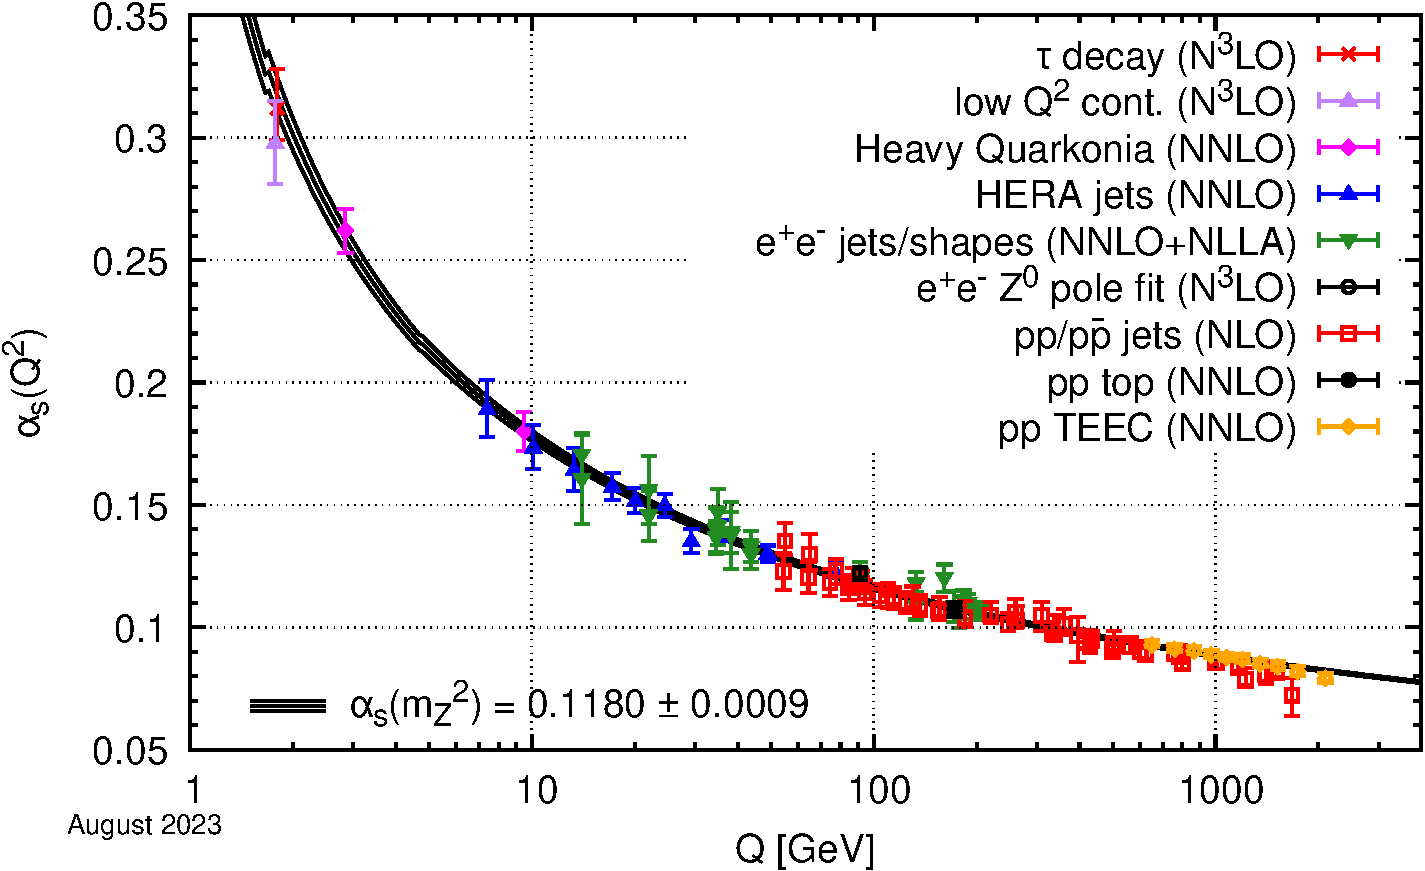
\includegraphics[width=0.6\linewidth]{2_theory/alphas}
    \caption{Medidas experimentales de la constante de acoplamiento de \ac{QCD} comparada con las predicciones calculadas a nivel de 5 loops~\cite{ParticleDataGroup2024}.}
    \label{fig:theory:sm:mathematical:qcd:alphas}
\end{figure}


\paragraph{Confinamiento y libertad asintótica}

Se dice que la constante de acoplamiento \textit{corre}, siendo grande a baja energía y haciéndose más pequeña a alta energía. De la \Eqn{\ref{eq:theory:sm:mathematical:qcd:alphas}}, a altas energías \(\alpha_s \to 0\) y en consecuencia, los quarks se comportan como partículas no acotadas, fenómeno conocido como libertad asintótica~\cite{Wilczek_Gross-1973,Politzer-1973}.
Por otro lado, para bajas energías (\(Q^2 \to 0\)), el acoplamiento \(\alpha_s\) aumenta divergentemente y por tanto \ac{QCD} da lugar al confinamiento de quarks y gluones~\cite{Glashow_Georgi-1974}. El confinamiento implica que ni los quarks ni los gluones pueden aparecer aislados sino que forman compuestos sin color llamados hadrones.
Además, a partir de la escala de corte infrarroja \(\Lambda_{\text{QCD}}\), donde la aproximación perturbativa a \(\alpha_s\) ya no es válida, la creación de pares quark-antiquark en el vacío es energéticamente más favorable que la separación de un par de quarks ligados. Por esta razón, a medida que pierden energía, los quarks y gluones producidos en un colisionador de protones sufren un proceso repetitivo conocido como hadronización, en el que se crean cascadas colimadas de hadrones, denominadas jets, que forman un cono desde el quark o gluón inicial.


\subsection{Interacciones hadrónicas en colisionadores protón-protón}
\label{subsec:theory:sm:hadron_interactions}

Como se discute en la \Sect{\ref{subsubsec:theory:sm:mathematical:qcd}}, la constante de acoplamiento \(\alpha_s\), que gobierna las interacciones fuertes entre quarks, tiene una fuerte dependencia de la escala de energía de cada interacción, modificando radicalmente la naturaleza de los procesos. La modelización de una colisión protón-protón en un experimento como lo es \ac{ATLAS}, en el que es necesario conocer su evolución desde la interacción entre los protones a \(\sqs \sim \tev\), hasta la interacción de las partículas en el estado final con los materiales activos y pasivos del detector a unos pocos GeV, representa un enorme reto ya que abarca regímenes de comportamiento \ac{QCD} muy diferentes. Dado que el \ac{LHC} es un colisionador de protones es importante disponer de una descripción muy precisa de la estructura de los protones, ya que una colisión \pp a muy altas energías consiste básicamente en colisionar los constituyentes de los mismos.

A energías muy altas, pero dentro del régimen perturbativo, la colisión entre dos protones puede estudiarse mediante el Modelo de Partones. Este modelo fue introducido por Feynman~\cite{Feynman-1969} y Bjorken~\cite{Bjorken-1969_1} a finales de los años 60 para interpretar la dispersión inelástica profunda electrón-núcleo en SLAC. Esta descripción ha demostrado ser una buena aproximación para interacciones partón-partón con gran transferencia de momento (es decir, el escalado de Bjorken~\cite{Bjorken-1969_2}), pero no es apropiada para modelizar la interacción a bajas energías.
Bajo esta abstracción, los partones incluyen no sólo los quarks de valencia (\(u\), \(\bar{u}\) y \(d\) en el caso del protón) sino también los pares de partículas y antipartículas en el mar de quarks y los gluones que median las interacciones entre ellos. El modelo asume una interacción permanente entre los partones, por lo que su momento individual es desconocido, aunque su fracción de momento con respecto al momento total del hadrón puede modelizarse como una variable aleatoria.
Además, en el caso de la verificación experimental, los quarks y gluones en el estado final no se observan directamente debido a la hadronización. En su lugar, se calcula una sección eficaz hadrónica efectiva, \(\sigma(\pp\to jj)\), entre los protones incidentes y los jets del estado final. Para realizar este paso, se utiliza el teorema de factorización~\cite{Ellis_Georgi_Politzer_Ross-1978,Feynman-1969,Collins_Soper_Sterman-book,Collins_Soper-1987}, que permite una separación sistemática entre las interacciones de corta distancia (de los partones) y las interacciones de larga distancia (responsables del confinamiento del color y de la formación de hadrones). Este teorema establece que la sección eficaz total para dos hadrones puede obtenerse ponderando y combinando las secciones eficaces para dos partones particulares. Esta ponderación se realiza utilizando lo que se conoce como una \ac{PDF1}, \(f_i(x,Q^2)\), que describe la densidad de partones para un partón de la especie \(i\) en un hadrón, con una fracción \(x\) de la energía-momento del hadrón cuando el hadrón se prueba a una escala de \(Q^2\). La sección eficaz para un proceso de dispersión dura \(\pp \to X\), iniciado por dos hadrones con cuadrimomentos \(P_1\) y \(P_2\) puede escribirse como:
\begin{equation}
    \label{eq:theory:sm:hadron_interactions:xs}
    \sigma_{\pp\to X} = \sum_{ij} \int_0^1 \dd{x_1} \dd{x_2} f_i(x_1, \mu_F^2) f_j(x_2, \mu_F^2) \, \hat{\sigma}_{ij}\left(p_1, p_2, \alpha_s(\mu_R^2), Q^2/\mu_R^2, Q^2/\mu_F^2 \right),
\end{equation}
donde \(x_1\) y \(x_2\) son las fracciones de momento transportadas por los partones interactuantes, y \(p_1 = x_1 P_1\) y \(p_2 = x_2 P_2\) son los momentos de los partones interactuantes. La sección eficaz partonica \(\hat{\sigma}_{ij}\), correspondiente a la interacción de los partones \(i\) y \(j\), se calcula a un orden fijo en \(\alpha_s\), que se evalúa a una cierta escala de renormalización \(\mu_R\) y escala de factorización \(\mu_F\). La escala de renormalización \(\mu_R\) es importante para absorber las divergencias \ac{UV} en los cálculos a órdenes superiores. La sección eficaz total se obtiene sumando todos los posibles sabores de partón e integrando todas las posibles fracciones de momento. Las \acp{PDF1}, \(f_i\) y \(f_j\), se evalúan a una escala de factorización, \(\mu_F\) , que puede considerarse como la escala que separa la física perturbativa de corta distancia de la física no perturbativa de larga distancia (es decir, separa los procesos duros de los blandos).

Si la expansión perturbativa se llevara a todos los órdenes, la sección eficaz en la \Eqn{\ref{eq:theory:sm:hadron_interactions:xs}} sería independiente de \(\mu_F\) y \(\mu_R\). Sin embargo, en el cálculo real de orden finito esto no es así. Suelen tomarse ambos como iguales, \(\mu_F = \mu_R = \mu\), elegidos a la escala típica \(Q^2\) del proceso, para minimizar la contribución de los términos de orden superior no calculados cuyas formas son logarítmicas \(\log\left(Q^2/\mu_R^2\right)\) y \(\log\left(Q^2/\mu_F^2\right)\). La dependencia de la predicción de \(\mu_R\) y \(\mu_F\) se asigna como incertidumbre teórica. El hecho de que la sección eficaz de un proceso deba ser independiente de la escala de factorización \(\mu_F\) condujo a las ecuaciones DGLAP (Dokshitzer-Gribov-Lipatov-Altarelli-Parisi)~\cite{Dokshitzer-1977,Gribov_Lipatov-1971,Altarelli_Parisi-1977}. Estas ecuaciones determinan la evolución de la \ac{PDF1} con \(Q^2\).
Para el caso del protón, la \Fig{\ref{fig:theory:sm:hadron_interactions:pdfs}} muestra las \acp{PDF1} evaluadas a dos escalas de factorización diferentes para todos los partones posibles.

\begin{figure}[ht!]
    \centering
    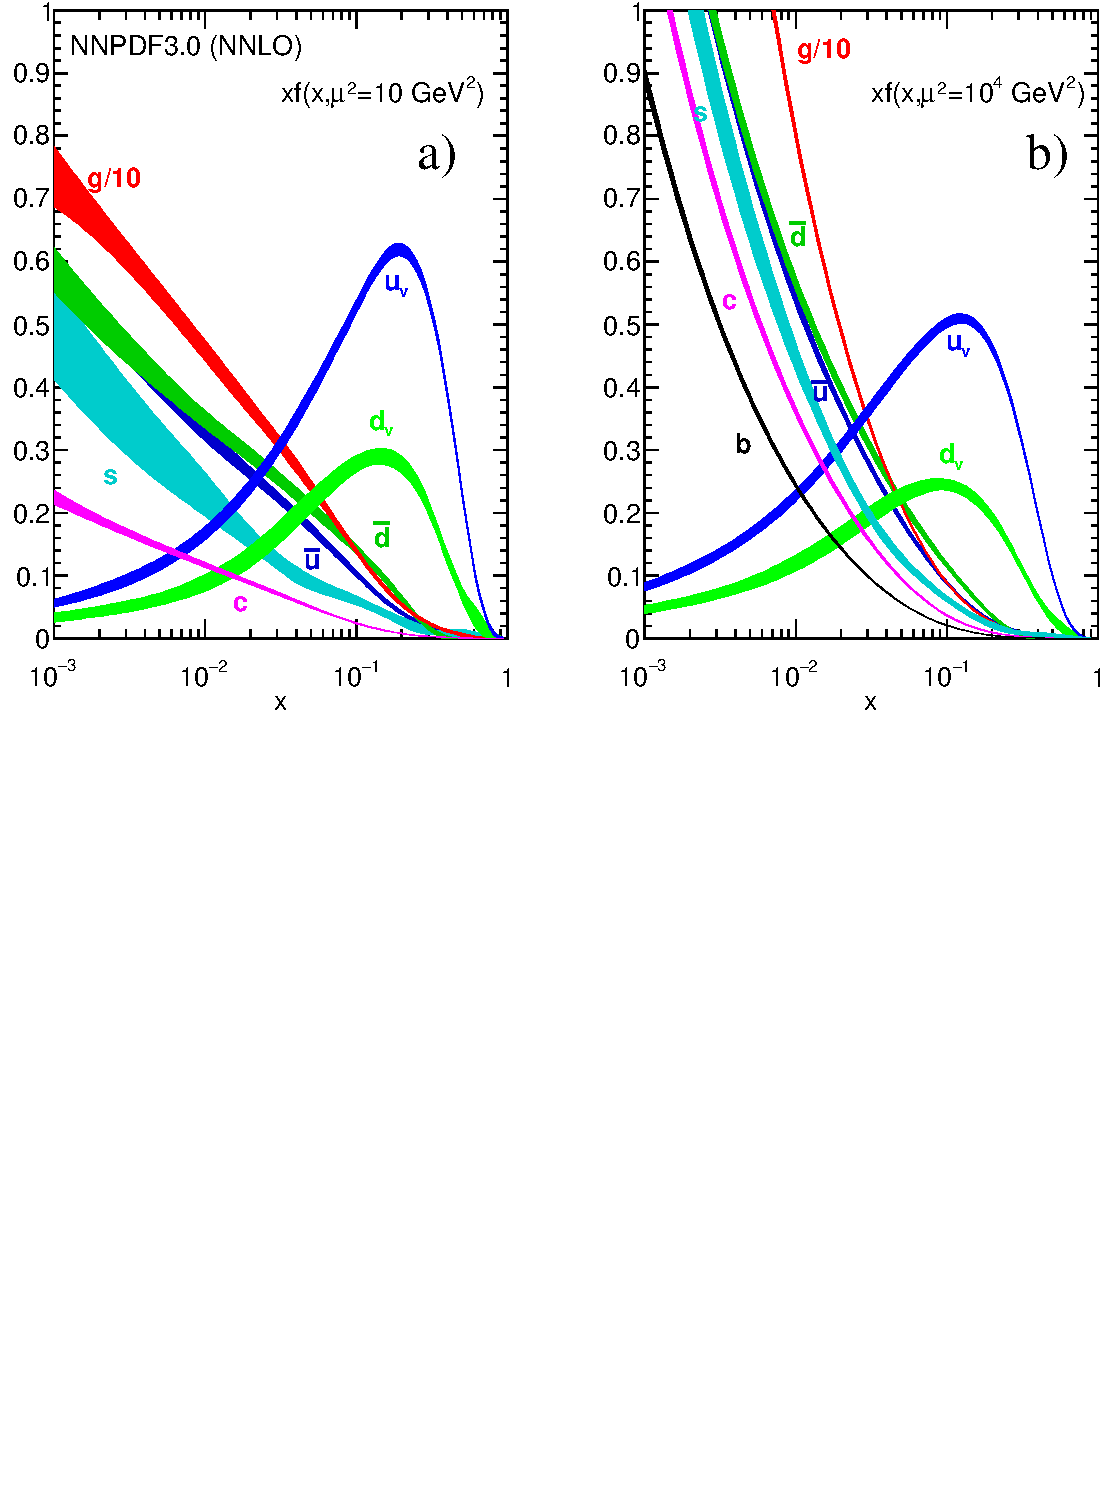
\includegraphics[width=0.7\linewidth]{2_theory/pdfs}
    \caption{Fracción del momento \(x\) del partón multiplicado por su correspondiente \acs{PDF1} \(f_i(x, Q^2)\) (donde \(i = u_v = u - \bar{u}, \, d_v = d - \bar{d},\, \bar{u},\, \bar{d},\, s\simeq\bar{s},\, c=\bar{c},\, b=\bar{b},\, g \)) obtenida por el análisis global a \ac{NNLO} NNPDF3.0~\cite{NNPDF} para dos escalas diferentes: \(\mu^2 = 10~\gev^2\) (izquierda) y \(\mu^2 = 10^4~\gev^2\) (derecha), utilizando \(\alpha_s(M_Z^2) = 0.118\). Las figuras son extraídas de la \Refn{\cite{ParticleDataGroup2020}}.}
    \label{fig:theory:sm:hadron_interactions:pdfs}
\end{figure}




\subsubsection{Descripción del proceso de colisión}

Inicialmente dos hadrones se acercan en un curso de colisión, donde cada hadrón puede pensarse como un grupo de partones esencialmente colineales caracterizados cuantitativamente por las \acp{PDF1}.
Se denomina como colisión dura a la colisión entre los dos partones procedientes uno de cada hadrón. Esta proceso puede ser calculado por una aproximación perturbativa hasta cierto orden en \(\alpha_s\).%, que corresponde al número de partones salientes.
En un escenario de colisión con partículas aceleradas que llevan carga \ac{EM} y cargas de color, procesos de bremsstrahlung pueden ocurrir antes y despues de la colisión dura, como por ejemplo radiación de gluones como \(q \to qg\).
Las emisiones que se inician a partir de los dos protones que colisionan se denominan \ac{ISR}, mientras que las radiaciones de los partones salientes se denominan \ac{FSR}. Con el desarrollo de la lluvia de partones, la intensidad del campo de \ac{QCD} aumenta (veáse la \Fig{\ref{fig:theory:sm:mathematical:qcd:alphas}}) a medida que los partones pierden energía y pueden romperse mediante la producción de pares quark-antiquark. Así, quarks y antiquarks pueden combinarse para producir un hadrón primario. La creación de hadrones como consecuencia del fenómeno de confinamiento se denomina \enquote{hadronización}. Los productos adicionales de la colisión que no están explícitamente relacionados con el proceso duro (radiación, restos de hadrones, productos de interacciones de múltiples partones, etc.), se suelen agrupar y denominar \ac{UE}. Una visualización de la colisión \pp se muestra en la \Fig{\ref{fig:theory:sm:hadron_interactions:parton_shower}}.



\begin{figure}[ht!]
    \centering
    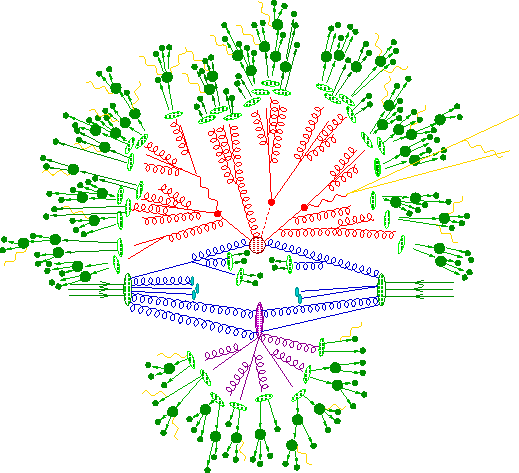
\includegraphics[width=0.7\linewidth]{2_theory/parton_shower}
    \caption{Ilustración de las etapas de una colisión hadrón-hadrón. El círculo rojo en el centro de la figura representa la colisión dura, rodeada por una estructura en forma de árbol que representa la radiación bremmstrahlung que simulan las \textit{parton showers}. El óvalo violeta en la parte inferior representa un ejemplo de un evento secundario de dispersión dura (\ac{UE}). El proceso de hadronización está representado por los óvalos verdes claro, mientras que los círculos verdes oscuro indican los decaimientos hadrónicos. Finalmente, las líneas amarillas señalan la radiación de fotones.~\cite{Hoche-2015}.}
    \label{fig:theory:sm:hadron_interactions:parton_shower}
\end{figure}



A lo largo de los años, diferentes experimentos del \ac{LHC} han medido secciones eficaces de diferentes procesos del \ac{SM}. La \Fig{\ref{fig:theory:sm:hadron_interactions:sm_results}} muestra la buena concordancia entre las secciones eficaces medidas por \ac{ATLAS} de algunos procesos y sus predicciones teóricas.


\begin{figure}[ht!]
    \centering
    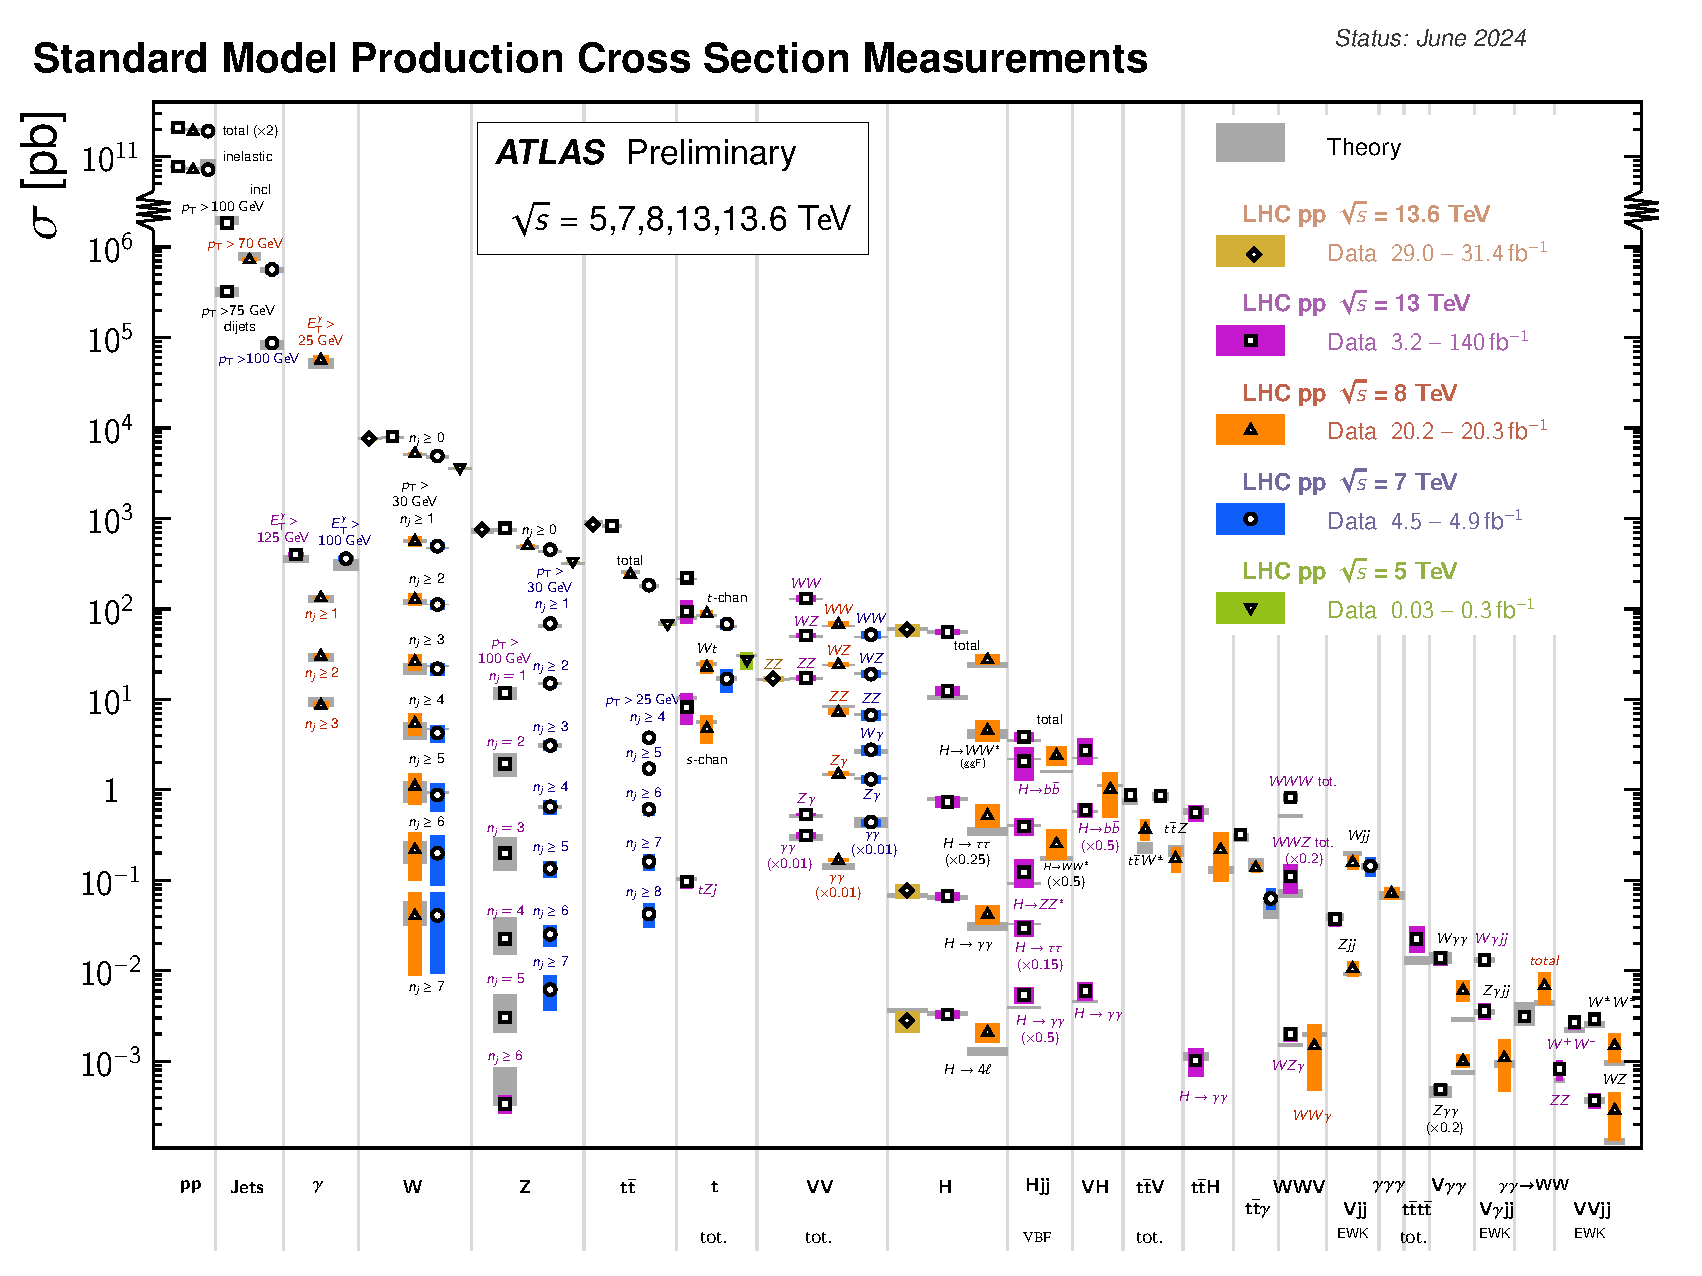
\includegraphics[width=0.8\linewidth]{2_theory/sm_measurements}
    \caption{Resumen de diversas medidas experimentales de las secciones eficaces de producción de diferentes procesos del \ac{SM}, comparadas con las predicciones teóricas~\cite{ATLAS-SM_Measurements}.}
    \label{fig:theory:sm:hadron_interactions:sm_results}
\end{figure}



\subsection{Teoría de producción de fotones \textit{prompt}}
\label{subsec:theory:sm:prompt_photon}


Los fotones de alto momento transverso originados en la colisión \pp (\enquote{prompt}) permiten investigar una gran variedad de procesos en escenarios de colisiones \pp, ya sea para realizar medidas de precisión del \ac{SM} o para llevar a cabo búsqueda de nueva física (\ac{BSM}). Una de las grandes ventajas de estos procesos es que las señales dejadas en los detectores por los fotones son mucho más limpias que las dejadas por jets, en donde además se cuenta con menores incertezas sistemáticas de reconstrucción e identificación.

% la interacción dura y su producción en colisiones protón-protón, \(\pp \to \gamma+X\), ofrece ciertas ventajas sobre otros análisis en eventos de producción de jets, el proceso más abundante en los colisionadores hadrónicos, proporcionando un escenario ideal para investigaciones sobre la teoría \ac{QCD}. En este caso, la presencia de un vértice \ac{QED} a \ac{LO} hace que los cálculos teóricos sean más confiables y da acceso a un rango más bajo de \pt. Además, la resolución energética de los calorímetros electromagnéticos es en general mejor que la de los calorímetros hadrónicos\footnote{Una descripción de ambos calorímetros se brinda en el \Ch{\ref{ch:atlas}}.}, y las incertidumbres sistemáticas en la escala de energía de los fotones son menores. Debido al hecho de que los fotones no hadronizan (véase \Sect{\ref{subsec:theory:mc_simulation:hadronisation}}), la dirección y la energía de los fotones se miden directamente en el calorímetro sin necesidad de contar con la reconstrucción de un jet.

La producción de fotones prompt tiene lugar a través de dos procesos: el proceso de fotones directos (D) en el que el fotón surge directamente de la interacción dura, y el proceso de fotones de fragmentación (F), en el que el fotón se emite en la fragmentación de un partón de alto momento transverso~\cite{Szczurek_Pietrycki-2007,Belghobsi_Fontannaz-2009}. Desde un punto de vista topológico, cuando se produce un fotón directo, generalmente está separado de la actividad hadrónica, mientras que un fotón producido a partir de un proceso de fragmentación, lo más probable es que esté acompañado de hadrones.

A \ac{LO} en teoría de perturbaciones, hay dos subprocesos que contribuyen a la producción de fotones directos: (a) el proceso Compton \(qg \to \gamma q\) y (b) el proceso de aniquilación \(\qqbar \to \gamma+g\), mostrados en las \Figs{\ref{fig:theory:sm:prompt_photon:feynman_lo_direct:compton}}{\ref{fig:theory:sm:prompt_photon:feynman_lo_direct:annihilation}}, respectivamente. A mediano y gran \(x\) (fracción de momento del partón) hay una jerarquía natural de distribuciones de partones en el protón, \(q \gg g \gg \bar{q}\), mientras que a pequeño \(x\), \(g \gg q,\bar{q}\) (\Fig{\ref{fig:theory:sm:hadron_interactions:pdfs}}). Como consecuencia, en las colisiones protón-protón, el proceso Compton \(qg\) domina esencialmente en todo el rango \pt. Esto hace que la producción prompt de fotones sea particularmente útil para restringir la distribución de gluones.

\begin{figure}[ht!]
    \centering
    \begin{subfigure}[h]{0.49\linewidth}
        \centering
        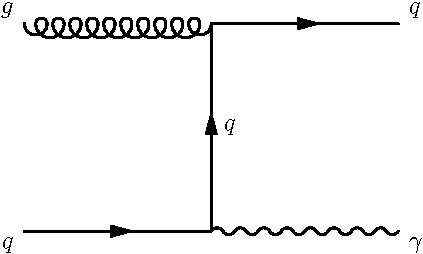
\includegraphics[width=0.7\linewidth]{2_theory/diagrams/gammajet_compton}
        \caption{Compton.}
        \label{fig:theory:sm:prompt_photon:feynman_lo_direct:compton}
    \end{subfigure}
    \hfill
    \begin{subfigure}[h]{0.49\linewidth}
        \centering
        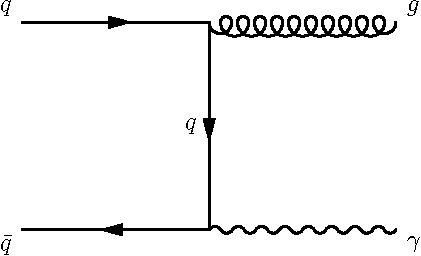
\includegraphics[width=0.7\linewidth]{2_theory/diagrams/gammajet_annihilation}
        \caption{Aniquilación.}
        \label{fig:theory:sm:prompt_photon:feynman_lo_direct:annihilation}
    \end{subfigure}
    \caption{Diagramas de Feynman de producción de fotones directos a \ac{LO} en colisiones \pp.}
    \label{fig:theory:sm:prompt_photon:feynman_lo_direct}
\end{figure}

Las correcciones a \ac{NLO} de este proceso se presentan en la \Fig{\ref{fig:theory:sm:prompt_photon:feynman_nlo_direct}}. En la \Fig{\ref{fig:theory:sm:prompt_photon:feynman_nlo_direct:gluon}}, existe una singularidad colineal cuando los momentos del quark y el gluón del estado final son paralelos. Esta divergencia se cancela cuando se suman las contribuciones real y virtual del gluón (un ejemplo de una contribución virtual se muestra en la \Fig{\ref{fig:theory:sm:prompt_photon:feynman_nlo_direct:gluon_virtual}}) y el efecto neto es una corrección finita \(\mathcal{O}(\alpha_s)\) al proceso \ac{LO}.

\begin{figure}[ht!]
    \centering
    \begin{subfigure}[h]{0.49\linewidth}
        \centering
        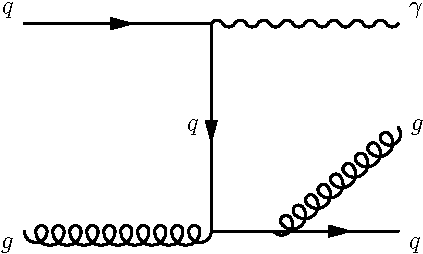
\includegraphics[width=0.7\linewidth]{2_theory/diagrams/gammajet_fsr_gluon}
        \caption{\Ac{FSR} de gluón.}
        \label{fig:theory:sm:prompt_photon:feynman_nlo_direct:gluon}
    \end{subfigure}
    \hfill
    \begin{subfigure}[h]{0.49\linewidth}
        \centering
        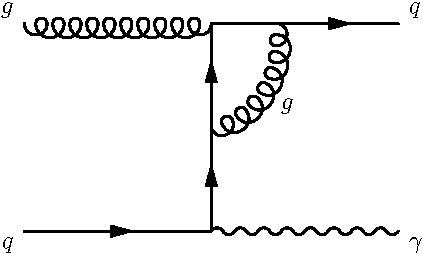
\includegraphics[width=0.7\linewidth]{2_theory/diagrams/gammajet_nlo_direct_virtualcorrection}
        \caption{Correcciones virtuales de gluones.}
        \label{fig:theory:sm:prompt_photon:feynman_nlo_direct:gluon_virtual}
    \end{subfigure}\\
    \caption{Diagramas de Feynman de producción de fotones directos a \ac{NLO} en colisiones \pp.}
    \label{fig:theory:sm:prompt_photon:feynman_nlo_direct}
\end{figure}

Asimismo, en la \Fig{\ref{fig:theory:sm:prompt_photon:feynman_nlo_frag}} se muestran las correcciones a la producción de fotones de fragmentación a \ac{NLO}. Al igual que para el caso de fotones directos, en los diagramas de las \Figs{\ref{fig:theory:sm:prompt_photon:feynman_nlo_frag:photon_fsr}}{\ref{fig:theory:sm:prompt_photon:feynman_nlo_frag:photon_isr}} se observan singularidades colineales pero, esta vez, cuando los momentos del fotón y del quark son paralelos. Esta singularidad, sin embargo, no se cancela sino que tiene que ser absorbida en una función de fragmentación de fotones \(D_q^{\gamma} (z, \mu^2_f )\) que representa la probabilidad de encontrar un fotón portando fracción de momento longitudinal \(z\) en un jet de quarks a escala \(\mu_f\). Estas correcciones a \ac{NLO} de la componente de fragmentación contiene también todos los procesos en los que un partón del estado final fragmenta para producir un fotón (dentro de la cascada partónica), incluido aquel donde el fotón es colineal al al momento del partón originario (\Figs{\ref{fig:theory:sm:prompt_photon:feynman_nlo_frag:quark}}{\ref{fig:theory:sm:prompt_photon:feynman_nlo_frag:gluon}}). Esta función de fragmentación no es calculable en teoría de perturbaciones y obedece a una ecuación de evolución DGLAP similar a la de las funciones de fragmentación hadrónicas. La contribución a la sección eficaz de la \Fig{\ref{fig:theory:sm:prompt_photon:feynman_nlo_frag}} contiene un factor de la forma
\begin{equation}
    \label{eq:theory:sm:prompt_photon:fragmentation_contribution}
    \hat{\sigma}(qg \to qg) \oplus D_q^{\gamma} \left(z, \mu_f^2\right).
\end{equation}
La función de fragmentación de fotones aumenta uniformemente con la escala en todo el rango de \(z\), es decir, \(D_k^{\gamma} \left(z, \mu_f^2\right) \sim d^{\gamma}(z)\ln(\mu^2)\) cuando \(\mu^2 \to \infty\). Cuando \(\pt \gtrsim \gev\), el crecimiento en la forma de \(\ln \pt^2\) de la función de fragmentación en la \Eqn{\ref{eq:theory:sm:prompt_photon:fragmentation_contribution}} compensa uno de los acoplamientos \(\alpha_s \left(\pt^2\right)\) en la sección eficaz del subproceso y la contribución es efectivamente de orden \(\alpha_s \left(\pt^2\right) \alpha_{EM}\), es decir, la misma que la contribución a \ac{LO}.


\begin{figure}[ht!]
    \centering
    \begin{subfigure}[h]{0.49\linewidth}
        \centering
        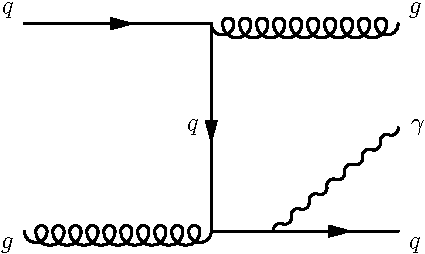
\includegraphics[width=0.7\linewidth]{2_theory/diagrams/gammajet_fsr}
        \caption{\Ac{FSR} de fotón.}
        \label{fig:theory:sm:prompt_photon:feynman_nlo_frag:photon_fsr}
    \end{subfigure}
    \hfill
    \begin{subfigure}[h]{0.49\linewidth}
        \centering
        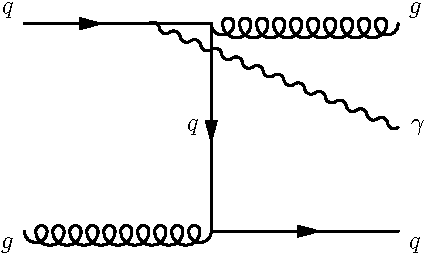
\includegraphics[width=0.7\linewidth]{2_theory/diagrams/gammajet_isr}
        \caption{\Ac{ISR} de fotón.}
        \label{fig:theory:sm:prompt_photon:feynman_nlo_frag:photon_isr}
    \end{subfigure}\\
    \begin{subfigure}[h]{0.49\linewidth}
        \centering
        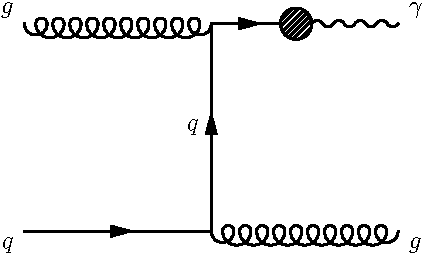
\includegraphics[width=0.7\linewidth]{2_theory/diagrams/gammajet_fragmentation_quark}
        \caption{Fragmentación de un fotón de un quark a \ac{NLO}.}
        \label{fig:theory:sm:prompt_photon:feynman_nlo_frag:quark}
    \end{subfigure}
    \hfill
    \begin{subfigure}[h]{0.49\linewidth}
        \centering
        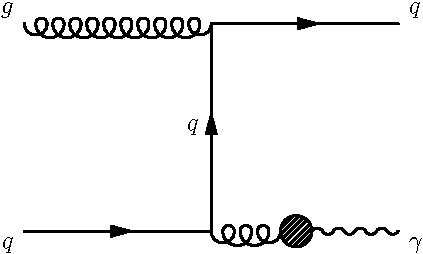
\includegraphics[width=0.7\linewidth]{2_theory/diagrams/gammajet_fragmentation_gluon}
        \caption{Fragmentación de un fotón de un gluón a \ac{NLO}.}
        \label{fig:theory:sm:prompt_photon:feynman_nlo_frag:gluon}
    \end{subfigure}\\
    \caption{Diagramas de Feynman de producción de fotones de fragmentación a \ac{NLO} en colisiones \pp.}
    \label{fig:theory:sm:prompt_photon:feynman_nlo_frag}
\end{figure}






La sección eficaz diferencial inclusiva en \(\etgam\) para la producción de un fotón no aislado viene dada por la suma de las contribuciones directas y de fragmentación:
\begin{align}
    \dv{\sigma}{\etgam} &= \dv{\sigma_{\text{dir}}}{\etgam} + \dv{\sigma_{\text{frag}}}{\etgam} \nonumber\\
    &= \sum_{a,b=q,\bar{q},g} \int \dd{x_a} \dd{x_b} f_a\left(x_a, \mu_F^2\right) f_b\left(x_b, \mu_F^2\right) \times \nonumber\\
    &\quad\quad
    \Biggl[
        \dd{\hat{\sigma}^{\gamma}_{ab} \left(p^{\gamma}; x_a, x_b, \mu_R, \mu_F, \mu_f\right)}
        + \nonumber\\
    &\quad\quad\quad\quad
    \sum_{c=q,\bar{q}, g} \int_{z_{\min}}^{1} \frac{\dd{z}}{z^2} \dd{\hat{\sigma}^c_{ab} \left(p^{\gamma}; x_a, x_b, z, \mu_R, \mu_F, \mu_f\right)} D_c^{\gamma} \left(z, \mu_f^2\right)
    \Biggr],
\end{align}
donde \(D_c^{\gamma} \left(z,\mu_f^2\right)\) es la función de fragmentación de un partón \(c\) a un fotón que lleva la fracción de momento \(z\), \(f_a \left(x_a, \mu^2_F \right)\) es la \ac{PDF1} de un partón \(a\), \(\mu_R\) y \(\mu_F\) son las escalas estándar de renormalización y factorización y \(\mu_f\) es la escala de fragmentación. Las correcciones de la componente directa de la sección eficaz partonica \(\hat{\sigma}^{\gamma}_{ab}\) se conocen hasta el \ac{NNLO} en \ac{pQCD}, mientras que la componente de fragmentación \(\hat{\sigma}^c_{ab}\) sólo se conoce a \ac{NLO}.

A \ac{LO}, los cálculos teóricos para los procesos directos y de fragmentación convergen por separado y pueden considerarse independientemente. Sin embargo, esta distinción no tiene significado físico más allá de \ac{LO}, ya que ambos tipos de procesos deben considerarse al mismo tiempo para cancelar las singularidades colineales e infrarrojas del estado final. Por lo tanto, más allá del \ac{LO}, tanto los procesos directos como los de fragmentación no pueden considerarse por separado. Desde un punto de vista teórico, la distinción viene definida por una elección arbitraria. Se deriva de la necesidad de factorizar las singularidades colineales del estado final y absorberlas en las funciones de fragmentación. Esta factorización requiere la introducción de una escala de fragmentación arbitraria \(\mu_f\), que es un parámetro no físico. En términos más generales, depende de la elección arbitraria del esquema de factorización, que define la parte finita de las correcciones de orden superior que se absorbe en las funciones de fragmentación junto con las singularidades; la parte finita restante se incluye entonces en las contribuciones de orden superior a las secciones eficaces partonicas. La dependencia de esta arbitrariedad y, en particular, de \(\mu_f\) se cancela sólo en la suma de las contribuciones directas y de fragmentación, por lo que sólo esta suma es un observable físico.






\section{Física Más allá del Modelo Estándar}
\label{sec:theory:bsm}

En la sección anterior se han descripto brevemente el \ac{SM}, junto con resultados de \ac{ATLAS} que muestran un muy buen acuerdo del \ac{SM} con los datos experimentales. A pesar de ser una de las teorías más exitosas de la física en general, el modelo tiene naturalmente un rango de validez.
Sin embargo, no puede considerarse la teoría definitiva ya que tiene ciertas limitaciones tanto desde el punto de vista teórico como experimental. El \ac{SM} se sigue considerando una teoría efectiva, una aproximación a baja energía de una teoría más fundamental. Hay tres tipos populares de teorías de la nueva física: (i) modelos con una simetría extendida o sector escalar, (ii) teoría de mayores dimensiones y (iii) fermiones compuestos (es decir, los fermiones del \ac{SM} ya no son elementales~\cite{Kuhn_Zherwas-1984,Cabibbo_Maiani_Srivastava-1984,DeRújula_Maiani_Petronzio-1984,Baur_Spira_Zerwas-1990,Bhattacharya_Chauhan_Choudhary_Choudhury-2009,Zhan_Li_Liu_Li-2016}).
A continuación, se presenta una vista general de las principales deficiencias del \ac{SM}. Luego, se discuten los modelos teóricos utilizados en la búsqueda llevada a cabo en esta tesis, que permiten resolver algunas de las cuestiones que el \ac{SM} no puede responder.

\begin{itemize}
    \item \underline{Gravedad:} Una de las principales limitaciones del \ac{SM} es la imposibilidad de incluir la gravedad del mismo modo que otras interacciones. No sólo incluir la gravedad en la teoría no es suficiente para explicar las observaciones, sino que las teorías matemáticas utilizadas en el \ac{SM} son prácticamente incompatibles con la formulación de la Relatividad General.
    \item \underline{Problema de jerarquías:} En el contexto de la física de altas energías se produce un problema de jerarquía cuando el valor fundamental de algún parámetro físico (como una constante de acoplamiento o una masa) en algún Lagrangiano es enormemente diferente de su valor efectivo, que es el valor que se mide en un experimento. Normalmente, el valor renormalizado de los parámetros se aproxima a sus valores fundamentales y, en general, los problemas de jerarquía están relacionados con el ajuste fino de los parámetros en la teoría. En física de partículas el problema de jerarquías es la diferencia entre la escala \ac{EW} \(M_W \sim 10^2~\gev\) y la escala de Planck, donde los efectos de la gravedad son relevantes \(M_P\sim10^{19}~\gev\), cuya relación es \(M_W / M_P \sim 10^{-17}\).
    \item \underline{\acf{DM}:} Una pista hacia la incompletitud del \ac{SM} es la presencia de \ac{DM}. Según mediciones astrofísicas y consideraciones cosmológicas~\cite{Zwicky-1937,Rubin_Kent-1970,Planck-2014,Clowe-2006,Brada-2008}, la materia conocida sólo representa menos del \(5\%\) del total del universo. Por otra parte, el \(23\%\) del total de la materia está asociado a un tipo de materia desconocida, denominada \ac{DM}, ya que no absorbe radiación \ac{EM}, pero es masiva al tener efectos gravitatorios considerables sobre la materia visible. La única partícula del \ac{SM} que podría ser un candidato \ac{DM} viable es el neutrino, pero como su masa es demasiado pequeña para explicar estos fenómenos, se ha descartado.
    \item \underline{Masa de los neutrinos:} La observación de la oscilación de los neutrinos implica que, aunque ellos tienen una masa muy pequeña, ésta no es nula, en contraste con la predicción del \ac{SM}. Aunque existen varios mecanismos para incluirlos en el \ac{SM}, no hay pruebas suficientes para saber cuál es la forma correcta y algunos modelos proponen la existencia de nuevas partículas pesadas aún no observadas~\cite{GellMann_Ramond_Slansky-2010,Glashow-1980,Ramond-2005}.
    \item \underline{Tres familias de fermiones:} El hecho de que sólo se hayan observado tres familias de fermiones también es uno de los gran interrogantes del \ac{SM} ya que no tiene ninguna explicación teórica. Como ya se ha mencionado, estas familias de quarks y leptones sólo difieren en la masa, mientras que todos los números cuánticos permanecen idénticos. Además, otro interrogante es por qué existen dos familias extras a las de la materia estable del Universo.
\end{itemize}





\subsection{Teorías de quarks compuestos}
\label{subsec:theory:bsm:qstar}

En las teorías de fermiones compuestos, éstos ya no son los constituyentes fundamentales de la materia sino estados ligados de partículas denominadas \textit{preones}~\cite{Pfeil-1981}. Se postula que estas últimas experimentan una fuerza desconocida hasta ahora a causa de una interacción de gauge asintóticamente libre pero confinante~\cite{Hooft-1980}, que se hace muy fuerte a una escala característica \(\Lambda\), dando lugar así a los fermiones compuestos. En muchos de estos modelos~\cite{Pati_Salam_Strathdee-1975,Fritzsch_Mandelbaum-1981,Baur_Fritzsch-1984}, aunque no en todos, los quarks y los leptones comparten al menos algunos constituyentes comunes. Tal hipótesis conduce naturalmente a la existencia de estados excitados de fermiones a una escala de masa comparable a la dinámica de la nueva interacción. Además, estos modelos brindan una solución al problema de las 3 generaciones de fermiones del \ac{SM}, dado que estas generaciones serían diferentes configuraciones o estados excitados de los preones.

Como los \enquote{estados excitados} sí sufren las interacciones de gauge del \ac{SM}, pueden producirse en colisionadores que operen a energías suficientemente altas. Al producirse, decaerían en partículas del \ac{SM} siendo un canal particularmente favorable el decaimiento radiativo en un fermión y un bosón gauge (fotón, \Wboson, \Zboson, o gluón). Si los quarks y los leptones no son constituyentes fundamentales sino que son compuestos, este hecho podría, en principio, revelarse mediante un exceso de datos a escalas de energía comparables a la escala de composición \(\Lambda\) en las colisiones \pp en el \ac{LHC}. Si el valor de \(\Lambda\) no es demasiado alto, entonces se pueden producir \ac{EQ} \textit{on-shell}, mientras que a energías muy por debajo de \(\Lambda\), tales excitaciones podrían manifestarse a través interacciones de contacto de cuatro fermiones que involucrara sólo partículas del \ac{SM}.

En general, las interacciones entre los \acp{EQ} (\qstar) y los bosones gauge pueden escribirse como~\cite{Zhan_Li_Liu_Li-2016}:
\begin{equation}
    \mathcal{L}_{\text{gauge}} = 
    \frac{1}{2\Lambda}
    \overline{\qstar_R}
    \sigma^{\mu\nu}
    \left[
        g_s f_s \frac{\lambda_a}{2} G_{\mu\nu}^a +
        g f \frac{\tau}{2} W_{\mu\nu} +
        g' f' \frac{Y}{2} B_{\mu\nu} +
    \right]
    q_L
    + \text{H.c},
\end{equation}
donde \(G_{\mu\nu}^a\), \(W_{\mu\nu}\) y \(B_{\mu\nu}\) son los tensores de intensidad de campo de los campos gauge SU(3), SU(2) y U(1), respectivamente. Los coeficientes \(g_s\), \(g = e / \sin \theta\), \(g' = e / \cos \theta\) son los acoplamientos gauge fuerte y \ac{EW}, \(\lambda_a\) es la matriz de Gell-Mann, \(\tau\) es la matriz de Pauli y la hipercarga débil es \(Y = 1/3\), respectivamente. \(\Lambda\) es la escala de composición y \(f_s, \, f, \, f'\) son parámetros determinados por la dinámica de composición que representan la intensidad de las interacciones entre el \acp{EQ} y los campos del \ac{SM}. Los diagramas de Feynman de los canales \(s\) y \(t\), a \ac{LO}, para dicho proceso se presentan en la \Fig{\ref{fig:theory:bsm:diagrams}}. Finalmente, la amplitud del decaimiento de \acp{EQ} a un fotón y un quark puede calcularse a \ac{LO}~\cite{Zhan_Li_Liu_Li-2016} como:
\begin{equation}
    \Gamma\left(\qstar \to q \gamma\right) =
    \frac{1}{4}
    \alpha
    \left(f \tau_3 + f' \frac{Y}{2}\right)^2
    \frac{\mq^3}{\Lambda^2}.
\end{equation}
que aumenta con la masa \mq del \ac{EQ} si se considera \(\Lambda = \mq\).


\begin{figure}[ht!]
    \centering
    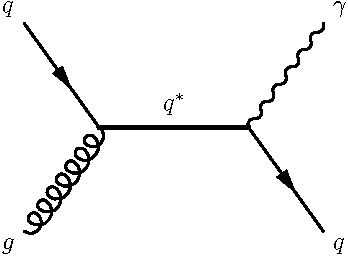
\includegraphics[width=0.3\linewidth]{2_theory/diagrams/qstar_gammajet_s_channel}
    \hspace{1cm}
    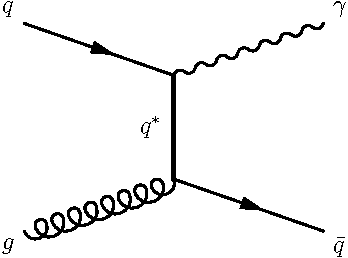
\includegraphics[width=0.3\linewidth]{2_theory/diagrams/qstar_gammajet_t_channel}
    \caption{Diagramas de Feynman de la producción de \ac{EQ} en colisiones \pp y su decaimiento en un quark y photon en el canal \(s\) (izquierda) y \(t\) (derecha).}
    \label{fig:theory:bsm:diagrams}
\end{figure}


En el \ac{SM} no hay un proceso de producción de una resonancia que decaiga en un par fotón+jet producido en colisiones \pp y la producción directa de fotón+jet a \ac{LO} ocurre vía dispersión Compton o aniquilación \qqbar, como se describió en la \Sect{\ref{subsec:theory:sm:prompt_photon}}. Como resultado, la distribución de la masa invariante \gammajet (\myj) cae rápidamente. De esta forma, un \ac{EQ} pesado que decae en un par \gammajet puede ser descubierto si existe. En lo que sigue de la tesis, de los modelos de \ac{EQ} que se estudian, sólo se considerarán los que decaen en un fotón y un jet. En el \Ch{\ref{ch:samples}} se da información sobre las secciones eficaces y las formas de las señales en el detector \ac{ATLAS}.

\subsection{Teorías con dimensiones extras}
\label{subsec:theory:bsm:qbh}

Explicar el problema de jerarquía, el enorme gap entre la escala \ac{EW} y la escala de Planck, ha sido una de las principales motivaciones para construir extensiones del \ac{SM}, como los modelos con supersimetría tecnicolor o de baja energía. Es notable que estas grandes estructuras teóricas, como lo son el \ac{SM} y la Teoría de Relatividad General, se hayan construido sobre el supuesto de la existencia de dos escalas de energía fundamentales muy dispares. Sin embargo, existe una diferencia importante entre estas escalas. Mientras que las interacciones \acp{EW} se han investigado a distancias cercanas a \(\sim m_W^{-1}\), las fuerzas gravitatorias no se han investigado ni remotamente a distancias \(\sim m_P^{-1}\).

Las propuestas de un espacio-tiempo con más de tres dimensiones espaciales se remontan a los años 20, principalmente a través de los trabajos de Kaluza y Klein, en un intento de unificar las fuerzas de la naturaleza~\cite{Bailin_Love-1987}. Aunque su idea inicial fracasó, el formalismo que ellos y otros desarrollaron sigue siendo útil hoy en día. Hacia 1980, la teoría de cuerdas propuso de nuevo ampliar el número de dimensiones espaciales, esta vez como requisito para describir una teoría coherente de la gravedad cuántica. Se suponía que las dimensiones extra se compactarían a una escala cercana a la de Planck por lo que no serían comprobables experimentalmente en un futuro próximo.

Arkani-Hamed, Dimopoulos y Dvali (ADD)~\cite{ADD-1998} dieron un enfoque diferente demostrando que la debilidad de la gravedad podría explicarse postulando dos o más dimensiones extra planas en las que sólo podría propagarse la gravedad. El tamaño de estas dimensiones extra debería oscilar entre aproximadamente un milímetro y \(\sim 1/\tev\), lo que daría lugar a posibles consecuencias observables en experimentos actuales y futuros. Otro enfoque, de Randall y Sundrum (RS)~\cite{RS1-1999_1,RS1-1999_2}, postula un espacio-tiempo Anti-deSitter (AdS) de cinco dimensiones con geometría deformada, donde la compactificación es de la escala de \(1/\tev\).

Estos modelos de gravedad de baja escala~\cite{Antoniadis_Arkani_Dimopoulos_Dvali-1998,ADD-1998,RS1-1999_1,RS1-1999_2,Dvali-2008,Dvali-2010} permiten la producción de \ac{QBH} en colisiones de partículas~\cite{Argyres-1998,Banks-1999,Giddings-2002}.
Los \ac{QBH}, a diferencia de los semiclásicos, muestran diferencias significativas a medida que su masa se aproxima a la escala de Planck. Los agujeros negros semiclásicos decaen térmicamente perdiendo masa a la temperatura de Hawking con un efecto mínimo en el espacio-tiempo circundante. Sin embargo, a medida que la masa del agujero negro disminuye y se acerca a la escala de Planck, la influencia de la reacción de retroceso en el espacio-tiempo se vuelve sustancial y el agujero negro ya no puede mantener el equilibrio térmico con su radiación. Cuando la longitud de onda Compton del agujero negro supera su radio de Schwarzschild, comienza a aparecer un comportamiento cuántico que podría conferirle propiedades similares a las de las partículas. En este punto, los conceptos de temperatura y entropía bien definidos ya no son válidos, lo que hace improbable que estos agujeros negros decaigan térmicamente~\cite{Meade-2008,Alberghi-2006,Alberghi-2007}.

Centrándose en agujeros negros con una masa ligeramente superior a la escala de Planck, se espera que los decaimientos de los \ac{QBH} no sigan un patrón térmico. En su lugar, es probable que dominen los decaimientos en unas pocas partículas y que estos procesos tengan lugar en una pequeña región del espacio-tiempo. Un \ac{QBH} podría comportarse como una resonancia fuertemente acoplada o un estado ligado gravitatoriamente.
% Tras el decaimiento del agujero negro, tendrá lugar el proceso de hadronización \ac{QCD}, dada la implicación de cargas de color.

En colisiones \pp, sólo una fracción de la energía total del centro de masa \sqs está disponible en el proceso de dispersión dura. Definiendo \(sx_ax_b \equiv s \tau \equiv \hat{s}\), donde \(x_a\) y \(x_b\) son las energías fraccionarias de los dos partones que colisionan (ver la \Sect{\ref{subsec:theory:sm:hadron_interactions}}), la sección eficaz completa \(\sigma\) se lee~\cite{Gingrich_Undseth-2020}:
\begin{equation*}
    \sigma_{\pp \to \text{BH} + X}(s) =
    \sum_{a,b}
        \int_{m^2/s}^{1} \dd{\tau}
            \int_{\tau}^{1}
            \frac{\dd{x}}{x}
            f_a\left(\frac{\tau}{x}\right)
            f_b(x)
            \Theta\left(m - m_{\text{th}}\right)
            \hat{\sigma}_{ab\to \text{BH}} (\hat{s} = m^2),
\end{equation*}
donde \(a\) y \(b\) recorren todos los partones y \(f_a\) y \(f_b\) son sus \acp{PDF1}. La función escalón de Heaviside \(\Theta\) marca el umbral de masa mínima \(m_{\text{th}}\) en el que se podría producir un \ac{QBH}.
Para un \ac{QBH}, el rango global en el que se considera que se producen es \(m_P \leq m \leq 3m_P\)~\cite{Gingrich-2010}.
La sección eficaz a nivel de partón \(\hat{\sigma}\) se considera a menudo como la sección eficaz geométrica \(\sigma \sim \pi r_g^2\) con
\begin{equation*}
    r_g = k(D) \frac{1}{m_P} \left(\frac{m}{m_P}\right)^{\frac{1}{D-3}},
\end{equation*}
donde \(k(D)\) es un coeficiente numérico que depende sólo del número de dimensiones y de la definición de la escala fundamental de Planck:
\begin{equation*}
    k(D) = 
    \left(
        2^{D-4}
        \left(\sqrt{\pi}\right)^{D-7}
        \frac{\Gamma \left(\frac{D-1}{2}\right)}{D-2}
    \right)
    ^{\frac{1}{D-3}}
\end{equation*}

Si la escala de Planck es lo suficientemente baja, los \ac{QBH} pueden producirse en abundancia en el \ac{LHC} y aparecerían como resonancias en la masa invariante de las partículas del estado final. Con respecto sólo al estado final \gammajet, hay seis estados de agujero negro no térmico posibles:
\begin{alignat*}{2}
    u + g       & \to QBH^{2/3}     && \to u + \gamma\\
    \bar{d} + g & \to QBH^{1/3}     && \to \bar{d} + \gamma\\
    q + \bar{q} & \to QBH^{0}       && \to g + \gamma\\
    q + g       & \to QBH^{0}       && \to g + \gamma\\
    d + g       & \to QBH^{-1/3}    && \to d + \gamma\\
    \bar{u} + g & \to QBH^{-2/3}    && \to \bar{u} + \gamma,
\end{alignat*}
donde \(u\) representa todos los quarks de tipo up, \(d\) todos los quarks de tipo down y \(q\) todos los sabores de quark. Al igual que en el modelo \ac{EQ}, en el \Ch{\ref{ch:samples}} se ofrece una descripción más detallada de los modelos, incluyendo su sección eficaz de producción.












\section{Simulaciones Monte Carlo}
\label{sec:theory:mc_simulation}


% La técnica \ac{MC} es una forma de calcular integrales complejas mediante métodos numéricos. 
Las colisiones de alta energía entre partículas elementales producen normalmente estados finales complejos, poblados por muchos hadrones, leptones, fotones y neutrinos. La relación entre los estados finales y la descripción física subyacente no es sencilla debido a la falta de comprensión de la física y al hecho de que cualquier aproximación analítica no es factible debido a las grandes multiplicidades de partículas. Una dificultad adicional está relacionada con la necesidad de simular factores geométricos complicados que representan detectores, una situación rutinaria para la colaboración \ac{ATLAS}.
Los métodos \ac{MC} permiten generar eventos completos con partículas finales (es decir, hadrones, leptones y fotones), con el mismo comportamiento medio y las mismas fluctuaciones que los datos. Mientras que en los datos las fluctuaciones surgen del carácter mecánico cuántico de la teoría subyacente, en los generadores estas fluctuaciones son el resultado de la (cuasi)aleatoriedad del enfoque \ac{MC}.

Los principales aspectos de los eventos simulados son: la colisión dura, la lluvia de partones, la hadronización y los \acp{UE}, siguiendo el esquema mostrado en la \Fig{\ref{fig:theory:sm:hadron_interactions:parton_shower}}.
Los principales generadores de eventos \ac{MC} utilizados en esta tesis son \PYTHIA 8~\cite{Pythia8.1,Pythia8.2,Pythia8.3} y \SHERPA 2.2.2~\cite{Sherpa2.2}.

\subsection{Colisión dura y lluvia de partones}

Para describir un proceso \(2 \to n\) a partir del Lagrangiano de la teoría (donde \(n\) representa un número determinado de partones en el estado final), se utilizan los diagramas de Feynman que se evalúan utilizando sus reglas específicas para calcular el \ac{ME1}. A medida que aumenta el número de partones en el estado final, el número de diagramas de Feynman crece factorialmente, haciendo que los cálculos de orden superior sean un reto. Sin embargo, los procesos complejos pueden simplificarse factorizándolos en procesos centrales \(2 \to 2\), que se convolucionan con probabilidades de división de partones para aproximar los efectos de orden superior. Los programas de simulación que aplican este enfoque son, por ejemplo, \pythia y \Herwig. Estos utilizan cálculos perturbativos a \ac{LO} de \acp{ME1} de procesos \(2 \to 2\) e implementan procesos de orden superior \ac{QCD} a través de las llamados \ac{PS} de estado inicial y final~\cite{Sjostrand-2006,Dobbs-2004} para producir el equivalente de estados finales multipartónicos.

En un proceso duro con virtualidad \(Q^2\), los partones entrantes y salientes emiten gluones siguiendo un patrón en el que las emisiones divergen cuando los gluones se vuelven colineales con los quarks o cuando su energía desaparece. Las ramificaciones de gluones (\(g \to gg\)) muestran divergencias similares, mientras que \(g \to \qqbar\) no. Los programas de \ac{QCD} a \ac{NLO}, como \Sherpa y \POWHEG, deben hacer coincidir a las \acp{PS} con el cálculo de \ac{ME1} para evitar el doble cómputo de emisiones. Estas emisiones, ordenadas por virtualidad creciente, continúan hasta que coinciden con el \(Q^2\) del proceso duro. De forma similar, la \ac{FSR} disminuye la virtualidad de los partones hasta que se alcanza un límite inferior (\(Q^2_0 \equiv \Lambda_{\text{QCD}} \sim 1~\gev\)), más allá del cual la teoría de perturbaciones pierde relevancia y se produce la hadronización.

\subsection{Hadronización}
\label{subsec:theory:mc_simulation:hadronisation}

A medida que la evolución alcanza \(Q^2_0 = \Lambda_{\text{QCD}} \), la fase de \ac{PS} se trunca ya que las fuerzas de acoplamiento se vuelven significativas y se produce el confinamiento. Este fenómeno aún no puede describirse a partir de primeros principios y, por tanto, implica cierta modelización para transformar todos los partones con color salientes en hadrones blancos de una escala de masas típica de 1 GeV. La dinámica de esta evolución se absorbe generalmente en funciones de fragmentación que representan la probabilidad de que un partón se fragmente en un hadrón determinado del estado final. Muchos de estos hadrones primarios son inestables y siguen decayendo en varias escalas de tiempo. Los que tienen un tiempo de vida media relativamente largo tienen sus decaimientos visibles en el detector, o son estables. Existen varios modelos del proceso de hadronización que intentan conectar los resultados de la \ac{PS} y el espectro final de partículas observado. Estos modelos pueden complementarse y ajustarse mediante observaciones experimentales. La hadronización se describe comúnmente mediante el modelo de fragmentación de cuerdas de Lund~\cite{Anderson-1983} (como se implementa en \Pythia), o el modelo de fragmentación de clusters~\cite{Webber-1984} (como se implementa en \Herwig y \Sherpa). Esencialmente, el modelo de fragmentación de cuerdas de Lund supone un confinamiento lineal en el que se asume que la energía almacenada en el campo de color entre quarks y antiquarks aumenta linealmente con la separación de las cargas de color. Así, representa la fuerza del color mediante un potencial linealmente creciente a medida que se separan las cargas, por lo que puede romperse por la producción de nuevos pares quark-antiquark que apantallan los colores de los extremos. Entonces, quarks y antiquarks pueden combinarse para producir hadrones. El modelo de fragmentación de clusters se basa en la propiedad de preconfinamiento de color de los procesos de ramificación que supone que la separación de las cargas de color que forman un singlete están inhibidas. Tras el proceso perturbativo de bifurcación de partones, los gluones restantes se dividen en pares livianos \qqbar, y entonces los quarks y antiquarks vecinos pueden combinarse en singletes de color (clusters incoloros) con distribuciones de bajas masas y asintóticamente independientes de la escala del subproceso duro.


\subsection{Evento subyacente}

Además de la interacción dura generada por la simulación \ac{MC}, también es necesario tener en cuenta las interacciones entre los restantes protones en cada cruce de bunches. Esto se suele modelizar a través de la dispersión múltiple extra \(2 \to 2\) que se produce a una escala de unos pocos GeV. La modelización del \ac{UE} es crucial para reproducir con precisión el flujo de energía que acompaña a las dispersiones duras en los colisionadores hadrónicos. El \ac{UE} puede incluir interacciones duras adicionales y procesos blandos que no pueden calcularse perturbativamente. Estos se modelizan con parámetros que se ajustan a los datos experimentales.



\subsection{Tunes}

Debido a la naturaleza no-perturbativa, y por tanto incalculable, de gran parte de los procesos de la física blanda, como las aproximaciones de lluvia, hadronización y \ac{UE}, los generadores \ac{MC} contienen inevitablemente una serie de parámetros libres. Estos diferentes parámetros suelen ajustarse con datos procedentes de colisionadores. Un conjunto específico de parámetros elegidos para un generador \ac{MC} se denomina \enquote{tune}.
En general, a lo largo de esta tesis se utiliza el tune A14 para \Pythia A14~\cite{Pythia-A14Tune}.
El tune A14 se basa en el tune MONASH~\cite{MonashTune} de los autores de \Pythia, que utiliza datos de colisiones \ee para los parámetros de hadronización y datos de colisiones \pp del tipo \textit{minimum-bias} en el \ac{LHC} para restringir los parámetros sensibles a la radiación del estado inicial y el \ac{UE}. El tune A14 utiliza además una gran variedad de datos de \ac{ATLAS} sensibles a las interacciones de múltiples partones y \ac{ISR}/\ac{FSR}, e incluye jets construidos a partir de trazas y variables sensibles a la estructura interna del jet.


\subsection{Simulación del detector \acs{ATLAS}}

Para comparar directamente los datos recolectados con el detector \ac{ATLAS} con la predicción de eventos simulados del \ac{SM} y \ac{BSM}, hay que además simular la interacción de las partículas producidas con el material del detector.
El paquete de software \GEANT~\cite{Geant4} se utiliza para simular la interacción de las partículas producidas en colisiones \pp  con las diferentes partes del detector (el detector \ac{ATLAS} se describe en el \Ch{\ref{ch:atlas}}). \GEANT es un extenso paquete de simulación de partículas que gobierna todos los aspectos de la propagación de ellas a través de detectores, basándose en una descripción de la geometría de los componentes del detector y del campo magnético. Los procesos físicos incluyen, entre otros, ionización, Bremsstrahlung, conversiones de fotones, dispersión múltiple, centelleo, absorción y radiación de transición. El último paso consiste en la digitalización, que simula las salidas del detector en el mismo formato que los datos reales. Debido a la detallada y complicada geometría del detector \ac{ATLAS} y a la diversidad y complejidad de los procesos físicos implicados, el tiempo de cálculo consumido por evento es grande (\(\mathcal{O}\)(5 minutos)).

La simulación de un gran número de interacciones necesarias para imitar los datos obtenidos en \ac{ATLAS} es computacionalmente extensa. Especialmente la simulación de los desarrollos de las lluvias en los calorímetros consume una gran cantidad de CPU y tiempo de cálculo. Para muchas búsquedas \ac{BSM} hay que simular un gran número de parámetros que afectan a las masas de las nuevas partículas e interacciones predichas, por lo que se ha desarrollado una simulación \enquote{rápida}, parametrizada, del detector para hacer frente a esta gran demanda de simulación.

La llamada simulación AtlFast3 o AF3~\cite{ATLAS-AF3} (construida sobre AltFast2~\cite{ATLAS-AF2}) utiliza la simulación \GEANT~\cite{Geant4} para las interacciones en el \ac{ID} y el \ac{MS} (descriptos en el \Ch{\ref{ch:atlas}}), y se utilizan dos simulaciones parametrizadas del \ac{ECAL} y del \ac{HCAL}: FastCaloSim v2\footnote{La versión previa, AtlFast2, hacía uso de FastCaloSim~\cite{ATLAS-FastCaloSim} para simular el paso de partículas por los calorímetros.} y FastCaloGAN.
Las simulaciones paramétricas de la respuesta del calorímetro simulan la energía de una lluvia de partículas como un único paso basado en una parametrización subyacente en lugar de simular cómo cada partícula se propaga e interactúa dentro del volumen del calorímetro.

AtlFast3 introduce varias mejoras claves en comparación con AtlFast2. En concreto, AtlFast3 mejora significativamente cómo se simulan los depósitos de energía en las celdas del calorímetro. Estas mejoras abordan las limitaciones de AtlFast2, en el que las estructuras de los subclusters y las formas de las lluvias laterales no se describían completamente. Esta nueva generación también integra simulaciones parametrizadas mejoradas y un modelo de calorímetro más preciso, lo que conduce a una reconstrucción mejorada de objetos físicos como jets y energía transversa faltante. Estos cambios mejoran la concordancia entre la simulación rápida y los resultados de la simulación completa.
Además, AtlFast3 soporta algoritmos más avanzados para la simulación de trazas y calorímetros, lo que garantiza que se minimicen las discrepancias observadas en AtlFast2, como las imprecisiones en las formas de las lluvias y las fluctuaciones.